\documentclass[14pt]{beamer}
\usepackage{hyperref}
\usepackage{ulem}
\usepackage[T1]{fontenc}
\usetheme{Madrid}

%% Enable license helpers
\graphicspath{ {../cc_beamer/}{pictures/} }
%%%%%%%%%%%%%%%%%%%%%%%%%%%%%%%%%%%%%%%%%%%%%%%%%%%%%%%%%%%%%%%%
%% ccBeamer 0.1, 2007-07-02                                   %%
%% Written by Sebastian Pipping <webmaster@hartwork.org>      %%
%% ---------------------------------------------------------- %%
%% Licensed under Creative Commons Attribution-ShareAlike 3.0 %%
%% http://creativecommons.org/licenses/by-sa/3.0/             %%
%%%%%%%%%%%%%%%%%%%%%%%%%%%%%%%%%%%%%%%%%%%%%%%%%%%%%%%%%%%%%%%%


%% Images
\newcommand{\CcImageBy}[1]{%
	
\includegraphics[scale=#1]{creative_commons/cc_by_30.pdf}%
}
\newcommand{\CcImageCc}[1]{%
	
\includegraphics[scale=#1]{creative_commons/cc_cc_30.pdf}%
}
\newcommand{\CcImageDevNations}[1]{%
	
\includegraphics[scale=#1]{creative_commons/cc_dev_nations_30.pdf}%
}
\newcommand{\CcImageNc}[1]{%
	
\includegraphics[scale=#1]{creative_commons/cc_nc_30.pdf}%
}
\newcommand{\CcImageNd}[1]{%
	
\includegraphics[scale=#1]{creative_commons/cc_nd_30.pdf}%
}
\newcommand{\CcImagePd}[1]{%
	
\includegraphics[scale=#1]{creative_commons/cc_pd_30.pdf}%
}
\newcommand{\CcImageSa}[1]{%
	
\includegraphics[scale=#1]{creative_commons/cc_sa_30.pdf}%
}
\newcommand{\CcImageSampling}[1]{%
	
\includegraphics[scale=#1]{creative_commons/cc_sampling_30.pdf}%
}
\newcommand{\CcImageSamplingPlus}[1]{%
	
\includegraphics[scale=#1]{creative_commons/cc_sampling_plus_30.pdf}%
}


%% Groups
\newcommand{\CcGroupBy}[1]{% zoom
	\CcImageBy{#1}%
}
\newcommand{\CcGroupByNc}[2]{% zoom, gap
	\CcImageBy{#1}\hspace*{#2}\CcImageNc{#1}%
}
\newcommand{\CcGroupByNcNd}[2]{% zoom, gap
	\CcImageBy{#1}\hspace*{#2}\CcImageNc{#1}\hspace*{#2}\CcImageNd{#1}%
}
\newcommand{\CcGroupByNcSa}[2]{% zoom, gap
	\CcImageBy{#1}\hspace*{#2}\CcImageNc{#1}\hspace*{#2}\CcImageSa{#1}%
}
\newcommand{\CcGroupByNd}[2]{% zoom, gap
	\CcImageBy{#1}\hspace*{#2}\CcImageNd{#1}%
}
\newcommand{\CcGroupBySa}[2]{% zoom, gap
	\CcImageBy{#1}\hspace*{#2}\CcImageSa{#1}%
}
\newcommand{\CcGroupDevNations}[1]{% zoom
	\CcImageDevNations{#1}%
}
\newcommand{\CcGroupNcSampling}[2]{% zoom, gap
	\CcImageNc{#1}\hspace*{#2}\CcImageSampling{#1}%
}
\newcommand{\CcGroupPd}[1]{% zoom
	\CcImagePd{#1}%
}
\newcommand{\CcGroupSampling}[1]{% zoom
	\CcImageSampling{#1}%
}
\newcommand{\CcGroupSamplingPlus}[1]{% zoom
	\CcImageSamplingPlus{#1}%
}


%% Text
\newcommand{\CcLongnameBy}{Attribution}
\newcommand{\CcLongnameByNc}{Attribution-NonCommercial}
\newcommand{\CcLongnameByNcNd}{Attribution-NoDerivs}
\newcommand{\CcLongnameByNcSa}{Attribution-NonCommercial-ShareAlike}
\newcommand{\CcLongnameByNd}{Attribution-NoDerivs}
\newcommand{\CcLongnameBySa}{Attribution-ShareAlike}

\newcommand{\CcNote}[1]{% longname
	This work is licensed under the \textit{Creative Commons #1 3.0 License}.%
}


\logo{
  
\includegraphics[scale=.1]{logo_buildtimetrend.png}
}
\title[Buildtime Trend]{Buildtime Trend}
\subtitle{What's trending in your build process}
\author{Dieter Adriaenssens}
\institute[]{Buildtime Trend founder \& developer - @dcadriaenssens}
\date[FOSDEM 2016]{FOSDEM 2016\\
January 31st, 2016}
\subject{Buildtime Trend}
\begin{document}
  \begin{frame}
    \titlepage
    \vfill
    \begin{center}
      \CcGroupByNcSa{0.83}{0.95ex}\\[2.5ex]
        {\tiny\CcNote{\CcLongnameByNcSa}}
        \vspace*{-2.5ex}
    \end{center}
  \end{frame}
  \begin{frame}
    \frametitle{Overview}
    \begin{itemize}
      \item What is Buildtime Trend?
      \item How does it work?
      \item How to start using it
      \item Demo
    \end{itemize}
  \end{frame}
  \begin{frame}
    \frametitle{What is Buildtime Trend?}
    Buildtime Trend is an Open Source application that uses (timing) data to visualise trends in a build process
  \end{frame}
  \begin{frame}
    \frametitle{It started with an itch}
    Project with unreliable builds on Travis CI:
    \begin{itemize}
      \item some builds took longer than others
      \item no timing information was present in the logs
      \item which stage took longer?
    \end{itemize}
  \end{frame}
  \begin{frame}
    \frametitle{Proof of concept}
    A script to generate a chart with duration of build stages :
    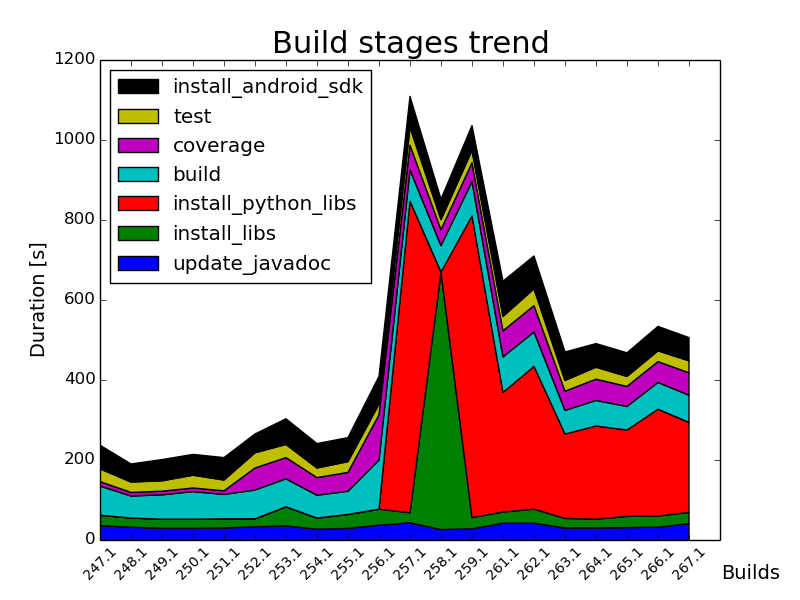
\includegraphics[scale=.45]{example_matplotlib_trend.png}
  \end{frame}
  \begin{frame}
    \frametitle{First release - dashboard}
    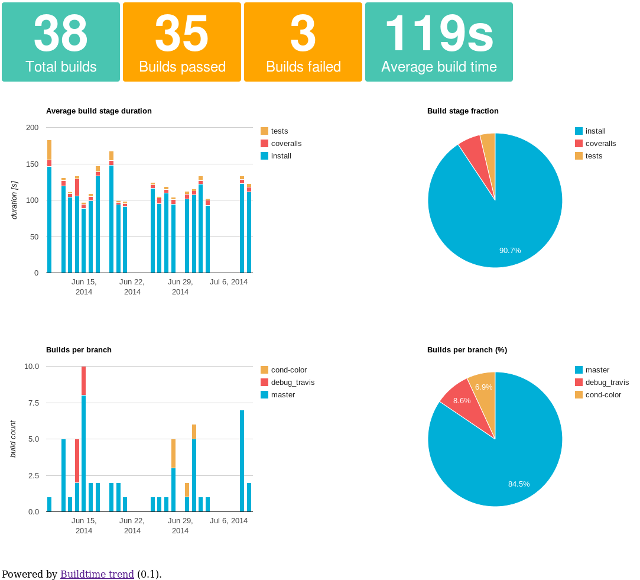
\includegraphics[scale=.45]{example_dashboard.png}
  \end{frame}
  \begin{frame}
    \frametitle{How it works}
    Webservice is triggered at the end of a build :
    \begin{itemize}
      \item download Travis CI build logfile
      \item parse the (timing) data
      \item store data
      \item visualise using a dashboard with charts
    \end{itemize}
  \end{frame}
  \begin{frame}
    \frametitle{Keen.io}
    
\includegraphics[scale=.20]{keenio_workflow.png}\\
    Keen IO's powerful APIs do the heavy lifting for you, so you can gather all the data you want and start getting the answers you need.
  \end{frame}
  \begin{frame}
    \frametitle{Hosting the service}
    \begin{itemize}
      \item CherryPy turns scripts into webservice
        \begin{itemize}
          \item dashboard
          \item badges
          \item buildjob log parser
        \end{itemize}
      \item service hosted on Heroku : \href{https://buildtimetrend.herokuapp.com/}{https://buildtimetrend.herokuapp.com/}
    \end{itemize}
  \end{frame}
  \begin{frame}
    \frametitle{How to use it}
    Trigger the service at the end of a Travis CI build in \textit{.travis.yml} :
    \begin{example}
      \small{notifications:\\
      \ \ webhooks:\\
      \ \ \ \ - https://buildtimetrend.herokuapp.com/travis}
    \end{example}
  \end{frame}
  \begin{frame}
    \frametitle{Who can use it}
    \begin{itemize}
      \item Webservice : free for Open Source (for now)
      \begin{itemize}
        \item \href{https://keen.io}{Keen.io} offered to host data for Open Source projects. \textbf{Thanks, guys!}
      \end{itemize}
      \item Source code available on Github
      \begin{itemize}
        \item service : host it yourself
        \item client : implement in your build process
      \end{itemize}
    \end{itemize}
  \end{frame}
  \begin{frame}
    \frametitle{Who is using it}
    \begin{itemize}
      \item Angular
      \item RocksDB (Facebook)
      \item phpMyAdmin
      \item Weblate
      \item MuseScore
      \item Servo
      \item pyca/cryptography
      \item Pootle
      \item \ldots
    \end{itemize}
  \end{frame}
  \begin{frame}
    \frametitle{Demo}
    \begin{itemize}
      \item Service : \href{https://buildtimetrend.herokuapp.com/}{\small{https://buildtimetrend.herokuapp.com/}}
      \item Badges : \href{https://github.com/buildtimetrend/service\#badge-examples}{\small{https://github.com/buildtimetrend/service\#badge-examples}}
    \end{itemize}
  \end{frame}
  \begin{frame}
    \frametitle{Future development}
    \begin{itemize}
      \item more and improved metrics and charts
      \item improve navigation and searching on dashboard
      \item support other CI platforms (Jenkins, ...)
      \item notifications
    \end{itemize}
  \end{frame}
  \begin{frame}
    \frametitle{Contributions welcome}
    \begin{itemize}
      \item use and test the service
      \item report bugs
      \item suggest improvements
      \item clone the project and send pull requests
      \begin{itemize}
        \item implement a feature
        \item fix a bug
        \item add a new chart
        \item improve dashboard layout
        \item \ldots
      \end{itemize}
    \end{itemize}
  \end{frame}
  \begin{frame}
    \frametitle{Acknowledgements}
    Big thanks to
    \begin{itemize}
      \item The nice people of Keen.io, for their invaluable support!
      \item the Open Source projects testdriving the service
      \item all the \href{https://github.com/buildtimetrend/python-lib/wiki/Credits}{services} that power the project
    \end{itemize}
  \end{frame}
  \begin{frame}
   \frametitle{Questions}
    Thanks for your attention!\\
    \vfill
    \href{https://twitter.com/dcadriaenssens}{\small{@dcadriaenssens}}
    \vfill
    Presentation available on \href{https://ruleant.github.io/presentations/}{\small{https://ruleant.github.io/presentations/}}
    \vfill
    Buildtime Trend
    \begin{itemize}
      \item Website : \href{https://buildtimetrend.github.io/}{\small{https://buildtimetrend.github.io/}}
      \item Service : \href{https://buildtimetrend.herokuapp.com/}{\small{https://buildtimetrend.herokuapp.com/}}
      \item Twitter : \href{https://twitter.com/buildtime_trend}{\small{@buildtime\_trend}}
    \end{itemize}
  \end{frame}
\end{document}
